\documentclass[11pt,xcolor=dvipsnames]{beamer}
\usetheme{nelle}
\usepackage{natbib}                 % Fancy bibliography.
\usepackage{url}                    % Allow printing of URLs.
\usepackage{outlines}
\usepackage{enumitem}
\usepackage{multicol}
\usepackage{dsfont}
\usepackage{amsmath}
\usepackage{epstopdf}
\usepackage{color}
\usepackage[utf8]{inputenc}
\usepackage{tikz}
\usetikzlibrary{decorations.pathreplacing,positioning, arrows.meta}

\setbeamerfont{caption}{size=\scriptsize}
\setbeamertemplate{navigation symbols}{}
\setbeamertemplate{footline}{%
\hfill\usebeamertemplate***{navigation symbols}
\raisebox{2pt}[0pt][0pt]{%
\color{gray}\hspace{1cm} \insertframenumber{} }
}

\def\newblock{\hskip .11em plus .33em minus .07em}

\title{\textbf{Machine learning in high dimension}\\
{\large Structures, functions, and regulations of genomes.}}
\subtitle{BCM-extended seminars}
\author[Varoquaux Nelle]{%
Nelle Varoquaux}
\date{November, 7th 2019}
\institute{CNRS, Teams GEM \& BCM, TIMC laboratory, Grenoble}

\begin{document}
\begin{frame}[t, noframenumbering]
  \maketitle
\end{frame}

\setcounter{framenumber}{0}


\begin{frame}
\frametitle{Nelle Varoquaux}

\begin{columns}
\begin{column}{0.8\linewidth}
{\bf \footnotesize In between computer science, statistics, and biology}
\vskip-1.3ex
\rule{\dimexpr\paperwidth-2.5cm\relax}{0.4pt}
\begin{itemize}[leftmargin=*]
\scriptsize
\item[-] 2010 Engineering degree {\bf Centrale Nantes} (Software engineering
\& CS)
\item[-] 2010-2011 Software engineer R\&D The pH Group, in London
\item[-] 2011-2012 M2 Master of applied mathematics, vision, and machine
learning{\bf ENS Cachan}
\item[-] 2012-2015 PhD {\bf Mines ParisTech}, CBIO team
\begin{itemize}
    \scriptsize
    \item[-] {\bf Developping statistical methods for analysing the 3D
    structure of the genome}
\end{itemize}
\item[-] 2016-2019 Postdoctoral researcher at {\bf UC Berkeley}, Department of
statistics
\begin{itemize}
    \scriptsize
    \item[-] {\bf Functional data analysis for time-course data} 
\end{itemize}
\end{itemize}

\begin{overlayarea}{10cm}{4cm}
\only<1->{%
{\bf \scriptsize Grants \& Awards}
\vskip-1.3ex
\rule{\dimexpr\paperwidth-3cm\relax}{0.4pt}
\begin{itemize}[leftmargin=*]
    \scriptsize
    \item[-] Moore-Sloan data science fellow at BIDS\quad
    \item[-] EMBER\quad Exploring maintainer burnout with ethnographic
    research\quad {\tiny (\$138 035) }
\end{itemize}

}
\only<1->{%
{\bf \scriptsize Scientific involvement}
\vskip-1.3ex
\rule{\dimexpr\paperwidth-3cm\relax}{0.4pt}
\begin{itemize}[leftmargin=*]
\scriptsize
\item[-] Organisation of conferences \& summer schools {\tiny (GraphXD, SciPy,
EuroScipy, Computational Reproducibility, ASPP \dots)}
\end{itemize}

\includegraphics[width=0.15\linewidth]{images/matplotlib.png} \quad

\includegraphics[width=0.12\linewidth]{images/scikit-learn.png} \quad

\includegraphics[width=0.15\linewidth]{images/scikit-image.png}
}
\end{overlayarea}


\end{column}
\begin{column}{0.08\linewidth}

\includegraphics[width=0.9\linewidth]{images/centrale_nantes.png} \\
\vspace{15pt}

\includegraphics[width=0.9\linewidth]{images/ens_cachan.png} \\
\vspace{15pt}

\includegraphics[width=0.9\linewidth]{images/ecole_des_mines.png} \\
\vspace{15pt}

\includegraphics[width=0.9\linewidth]{images/uc_berkeley.png} \\
\vspace{15pt}

\includegraphics[width=0.9\linewidth]{images/bids.png} \\
\vspace{15pt}

\includegraphics[width=0.9\linewidth]{images/moore_foundation.jpg} \\
\vspace{15pt}

\includegraphics[width=0.9\linewidth]{images/sloan_foundation.png}
\end{column}
\end{columns}

\end{frame}


\begin{frame}
\frametitle{Research path}
\vspace{4em}
\hspace{2em}
\begin{tikzpicture}[overlay]

% Main horizontal line
\draw[ultra thick,->] (-1cm,0) -- (7.5,0);

% draw vertical lines
\foreach \x in {0,2,4,6}
    \draw[ultra thick] (\x cm,3pt) -- (\x cm,-3pt);
\foreach \x in {1,3,5,7}
    \draw (\x cm,2pt) --(\x cm,-2pt);

% draw names
\draw[ultra thick] (0,0) node[below=3pt,thick] {2012} node[above=3pt] {};
\draw[ultra thick] (2,0) node[below=3pt,thick] {2014} node[above=3pt] {};
\draw[ultra thick] (4,0) node[below=3pt, thick] {2016} node[above=3pt] {};
\draw[ultra thick] (6,0) node[below=3pt, thick] {2018} node[above=3pt] {};

% Hi-C
\draw [thick] (0.5 cm,2pt) -- (0.5cm,1.5cm);
\draw [fill=red](0.5,0) circle (0.1cm);
\draw [thick] (0.5cm,1.5cm) -- (1cm,1.75cm);
\draw [thick] (1cm,1.5cm) -- (1cm,2cm);
\draw [thick] (1cm, 1.75cm) node[right=3pt] {\parbox[t]{3.5cm}{\scriptsize {\bf
{\em Analysing Hi-C data}}
\begin{itemize}[leftmargin=*]
\tiny
\item[-]{
\only<1-4>{%
\bf {\color{red} Varoquaux} et al., \scalebox{.7}{Bioinformatics (2014)}}
\only<5->{%
\bf \color{blue} Varoquaux et al., \scalebox{.7}{Bioinformatics (2014)}}
}
\item[-]{%
\only<1-4>{\bf Servant, {\color{red} Varoquaux} et al.
\scalebox{.7}{Genome Biology (2015)}}
\only<5->{\bf \color{blue} Servant, Varoquaux et al. \scalebox{.7}{Genome Biology (2015)}}
}
\item[-]{%
\only<1-4>{%
\bf {\color{red} Varoquaux} et al. \scalebox{.7}{NAR (2015)}}
\only<5->{%
\bf \color{blue} Varoquaux et al. \scalebox{.7}{NAR (2015)}}}
\item[-]{%
\only<1-4>{%
\bf Servant$^*$, {\color{red} Varoquaux$^*$} et al. \scalebox{.7}{BMC bioinformatics
(2018)}}
\only<5->{%
\bf \color{blue} Servant$^*$, Varoquaux$^*$ et al. \scalebox{.7}{BMC bioinformatics
(2018)}}
}
\item[-]{%
\only<1-4>{\bf {\color{red} Varoquaux}, Servant
\scalebox{.7}{JOSS (2019)}}
\only<5->{\bf \color{blue} Varoquaux, Servant \scalebox{.7}{JOSS (2019)}}}
\item[-]{%
\only<1-4>{%
\bf \color{gray}  {\color{red} Varoquaux} et al. \scalebox{.7}{(in prep.)}}
\only<5->{%
\bf \color{blue} Varoquaux et al. \scalebox{.7}{(in prep.)}}
}
\end{itemize}
}
};

% P. falciparum
\only<2->{
\draw [thick] (1 cm,2pt) -- (1cm,-3.25cm);
\draw [fill=red](1,0) circle (0.1cm);
\draw [thick] (1cm,-3.25cm) -- (1.5cm,-3.5cm);
\draw [thick] (1.5cm,-3.25cm) -- (1.5cm,-3.75cm);
\draw [thick] (1.5cm, -3.5cm) node[right=3pt] {\parbox[t]{5cm}{\scriptsize {\bf
\em 3D structure of P. falciparum}
\begin{itemize}[leftmargin=*]
\tiny
\item[-]{%
\only<1-4>{%
\bf Ay$^*$, Bunnik$^*$, {\color{red} Varoquaux$^*$} et al.,
\scalebox{.7}{Genome Research (2014)}}
\only<5->{%
\bf \color{green}Ay$^*$, Bunnik$^*$, Varoquaux$^*$ et al., \scalebox{.7}{Genome Research(2014)}}}
\item[-]{%
\only<1-4>{\bf Ay$^*$, Bunnik$^*$, {\color{red} Varoquaux} et al.
\scalebox{.7}{Bioessays (2014)}}
\only<5->{\bf \color{green} Ay$^*$, Bunnik$^*$, Varoquaux et al.
\scalebox{.7}{Bioessays (2014)}}}
\item[-]{%
\only<1-4>{\bf {\color{red} Varoquaux} \scalebox{.7}{International journal of
Biostatistics (2018)}}}
\only<5->{\bf \color{blue} Varoquaux \scalebox{.7}{International journal of
Biostatistics (2018)}}
\item[-] {%
\only<1-4>{\bf Bunnik$^*$, Cook$^*$, {\color{red} Varoquaux} et al.
\scalebox{.7}{Nature Communication (2018)}}
\only<5>{\bf \color{green}Bunnik$^*$, Cook$^*$, Varoquaux et al.
\scalebox{.7}{Nature Communication (2018)}}}
\end{itemize}
}
};
}
% EPICON
\only<3->{
\draw [thick] (4.5 cm,2pt) -- (4.5cm,-1.75cm);
\draw [fill=red](4.5,0) circle (0.1cm);
\draw [thick] (4.5cm,-1.75cm) -- (4.75cm,-2cm);
\draw [thick] (4.75cm, -1.75cm) -- (4.75cm,-2.25cm);
\draw [thick] (4.75cm, -1.75cm) node[right=3pt] {\parbox[t]{6cm}{\scriptsize {\bf
\em Functional data analysis \& gene expression}
\begin{itemize}[leftmargin=*]
\tiny
\item[-]{%
\only<1-4>{\bf Giordano$^*$, Liu$^*$, {\color{red} Varoquaux$^*$}, et
al. \scalebox{.7}{NIPS AABIW (2017)}}
\only<5->{\bf \color{blue} Giordano$^*$, Liu$^*$, Varoquaux$^*$, et
al. \scalebox{.7}{NIPS AABIW (2017)}}
}
\item[-]{%
\only<1-4>{%
\bf {\color{red} Varoquaux$^*$}, Cole$^*$, Gao$^*$ et al.
\scalebox{.7}{(accepted)}}
\only<5->{%
\bf \color{green} Varoquaux$^*$, Cole$^*$, Gao$^*$ et al
\scalebox{.7}{(accepted)}
}}
\item[-]{%
\only<1-4>{%
\bf \color{gray} {\color{red} Varoquaux}, Purdom \scalebox{.7}{(in prep.)}}
\only<5->{%
\bf \color{blue} Varoquaux, Purdom \scalebox{.7}{(in prep.)}}}
\item[-] {%
\only<1-4>{%
\bf \color{gray} {\color{red} Varoquaux$^*$}, DeGraaf$^*$ et al.
\scalebox{.7}{(in prep)}}
\only<5->{%
\bf \color{blue} Varoquaux$^*$, DeGraaf$^*$ et al. \scalebox{.7}{(in prep)}}}
\end{itemize}}
};}

% EMBeR
\only<4->{
\draw [thick] (5.5 cm,2pt) -- (5.5cm,0.5cm);
\draw [fill=red](5.5,0) circle (0.1cm);
\draw [thick] (5.5cm,.5cm) -- (5.75cm,0.75cm);
\draw [thick] (5.75cm, .5cm) -- (5.75cm,1cm);
\draw [thick] (5.75cm, 1cm) node[right=3pt] {\parbox[t]{5cm}{\scriptsize {\bf
\em Free and open-source software communities}
\begin{itemize}[leftmargin=*]
\tiny
\item[-]{%
\only<1-4>{\bf Geiger, {\color{red} Varoquaux} et al. \scalebox{.7}{(CSCW
2018)}}
\only<5->{\bf Geiger, Varoquaux et al. \scalebox{.7}{CSCW (2018)}}}
\item[-]{%
\only<1-4>{\bf \color{gray}  Paxton, {\color{red} Varoquaux} et al.
\scalebox{.7}{(in prep.)}}
\only<5->{\bf Paxton, Varoquaux et al. \scalebox{.7}{(in prep.)}}}
\end{itemize}
}
};}
%
\only<5->{%
\draw [thick] (7.5cm, -4.1cm) node[right=1pt] {%
\parbox[t]{5cm}{%
\fontsize{2.5}{4}
\tiny
\bf
{\color{blue} Methods development} \\
{\color{green} Collaborations in biology} \\
{\color{black} Collaborations in social sciences} \\
}};}

\end{tikzpicture}
\begin{overlayarea}{12cm}{2cm}
\vspace{-4cm}
\begin{flushright}
\only<4->{%

\includegraphics[width=0.15\linewidth]{images/matplotlib.png} \quad

\includegraphics[width=0.12\linewidth]{images/scikit-learn.png} \quad

\includegraphics[width=0.15\linewidth]{images/scikit-image.png} \quad
}
\end{flushright}
\end{overlayarea}

\end{frame}


\section{A statistical approach for inferring the 3D structure of the genome}  
\begin{frame}
\Large{ \bf
Statistical approaches for inferring the 3D structure of the genome.}

\begin{flushright}
\vspace{1em}
\small
\textit{joint work with A. Gesine Cauer, Gurkan Yardımcı, \\
Ferhat Ay, William S. Noble, \\ and Jean-Philippe Vert.}
\end{flushright}
\end{frame}

% 1. Motivation
\begin{frame}
\frametitle{Inferring 3D models of genome architecture from Hi-C data}
{\color{Blue} \textbf{Motivation}}
\begin{itemize}[label={$\bullet$}]
\item Little is known on the 3D structure of the genome.
\item Hi-C now allows to assess physical interactions genome-wide.
\end{itemize}

\vspace{1em}
{\color{Blue} \textbf{Goal}} Propose a robust and accurate method for
inferring 3D models of genome architecture from contact counts.

\vspace{1em}
{\color{Blue} \textbf{Idea}} Model contact counts as random variables
where the 3D model is a latent variable and cast the inference as maximizing
the likelihood.

\end{frame}


\begin{frame}
\frametitle{Inferring the 3D structure of the genome}

\begin{figure}
\centering
\includegraphics[width=0.5\linewidth]{images/counts_pfalc.pdf}
\end{figure}
\begin{flushright}
\tiny Ay$^*$, Bunnik$^*$, {\color{red} Varoquaux$^*$} et
al, Genome Research (2014)
\end{flushright}


\begin{overlayarea}{12cm}{4cm}
\only<2->{%
{\bf \small Hi-C data}
\footnotesize
\vskip-1.3ex
\rule{\dimexpr\paperwidth-1.5cm\relax}{0.4pt}
\begin{itemize}
\item[-] Very large matrices (human $3e10^6 \times
3e10^6$)
\item[-] Indirect and noisy measure of the 3D structure of the genome in a
population of cell
\end{itemize}
}
\end{overlayarea}
\end{frame}

\begin{frame}
\frametitle{Inferring the 3D structure of the genome}

\begin{overlayarea}{12cm}{4cm}
\only<1->{%
\begin{center}
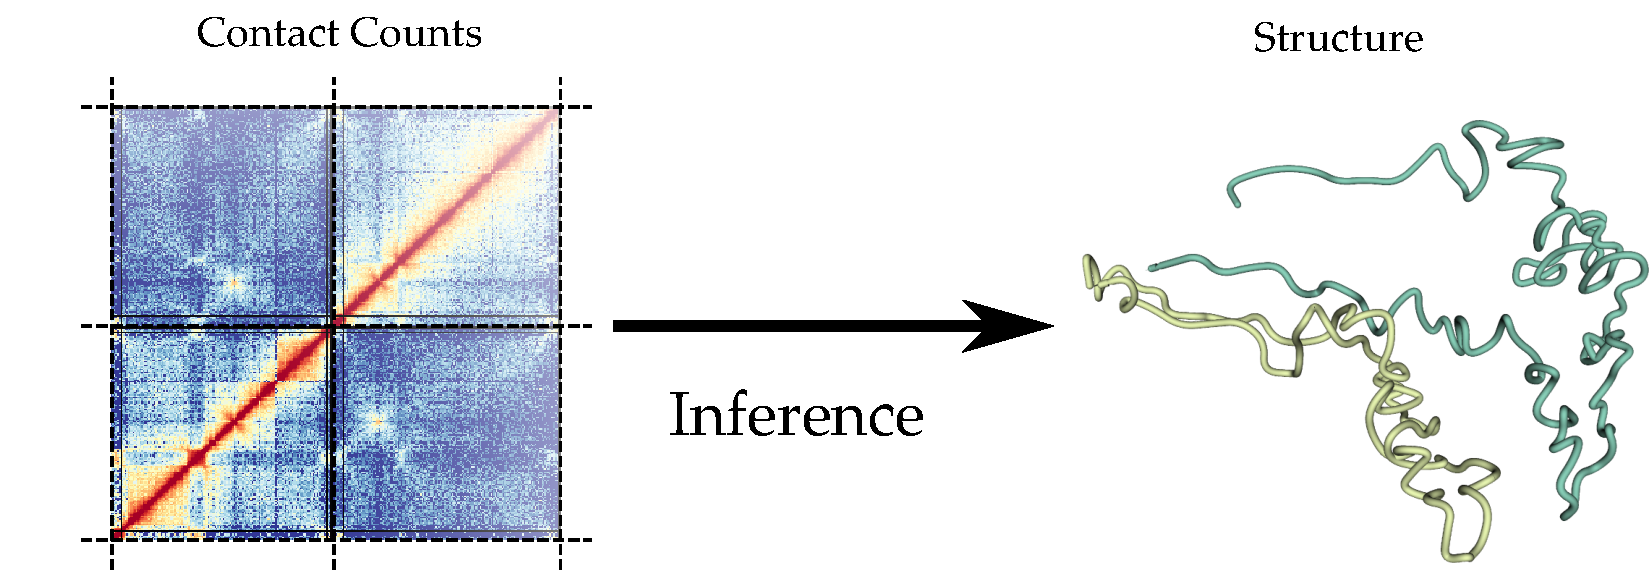
\includegraphics[width=0.9\linewidth]{figures/exemple_structure_inference.pdf}
\end{center}
}
\end{overlayarea}

\begin{overlayarea}{12cm}{4cm}
\only<2->{%
{\bf \small A statistical approach for inferring the 3D structure of the
genome}
\vskip-1.3ex
\rule{\dimexpr\paperwidth-1.5cm\relax}{0.4pt}
}
\only<2->{%
\begin{itemize}
\only<2>{%
\small
\item[-] Modelisation of the contact count between loci $i$ and $j$ :
{\large
\begin{equation*}
\underbrace{c_{ij}}_{\text{\tiny contact counts}} \sim
\quad
\text{Poisson}\Big(\underbrace{\beta_{ij}}_{\text{\tiny bias}}
\underbrace{\|x_i - x_j\|_2^\alpha}_{\text{\tiny distance}}\Big)
\end{equation*}}}
\only<3>{%
\small
\item[-] Likelihood maximization ($d_{ij} = \|x_i - x_j\|_2$)
  \begin{equation*}
  \underset{x_1, \dots x_n}{max} \ell(\mathbf{X}, \alpha, \beta) =
  \underset{i<j\leq n}{\sum} c_{ij} (\log(\beta 
  d_{ij} ^\alpha)) -  \beta d_{j}^\alpha
  \end{equation*}
}
\only<4>{%
\small
\item[-] Modelisation of the contact count between loci $i$ and $j$ :
{\large
\begin{equation*}
\underbrace{c_{ij}}_{\text{\tiny contact counts}} \sim
\quad
\text{NB}\Big(\underbrace{\beta_{ij}}_{\text{\tiny bias}}
\underbrace{\|x_i - x_j\|_2^\alpha}_{\text{\tiny distance}},
\underbrace{r(\|x_i - x_j\|_2, \beta_{ij}, \alpha)}_{\text{\tiny
dispersion}}\Big)
\end{equation*}}}
\only<5->{%
\small
\item[-] Likelihood maximization ($d_{ij} = \|x_i - x_j\|_2$)
  \begin{equation*}
  \hspace{-2.5em}
  \underset{x_1, \dots x_n}{\text{max}}\quad   \underset{i<j\leq n}{\sum}  \log\Big(\frac{\Gamma(c_{ij} +
  \beta_{ij} r(d_{ij}^\alpha))}{\Gamma(c_{ij} +
  1)\Gamma(\beta_{ij} r(d_{ij}^\alpha))} \Big(\frac{d_{ij}^\alpha}{r(d_{ij}^\alpha) + d_{ij}^\alpha}\Big)^{c_{ij}}
  \Big(\frac{r(d_{ij}^\alpha
  )}{r(d_{ij}^\alpha) + d_{ij}^\alpha}\Big )^{\beta_{ij}r(d_{ij}^\alpha)}\Big)
  \end{equation*}}
\end{itemize}
\vspace{-1em}
\begin{flushright}
{\tiny
{\color{red} Varoquaux} et al., Bioinformatics (2014)\\
Bunnik$^*$, Cook$^*$, {\color{red} Varoquaux} et al, Nature Communications (2018)\\
\vspace{-1em}
{\color{red} Varoquaux} et al., en préparation}
\end{flushright}}
\end{overlayarea}
\end{frame}

\begin{frame}
\frametitle{Inferring the 3D structure of diploid genomes}
\begin{overlayarea}{12cm}{4cm}
\begin{figure}
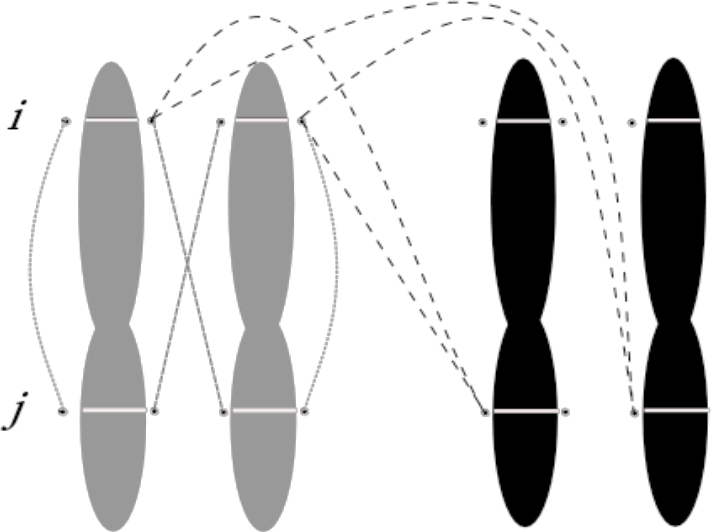
\includegraphics[width=0.3\linewidth]{images/counts_hic_diploid.png}
\end{figure}
\end{overlayarea}
\begin{overlayarea}{12cm}{4cm}
\only<2->{%
{\bf \small Modeling contact counts as sums of Poisson random variables}
\vskip-1.3ex
\rule{\dimexpr\paperwidth-1.5cm\relax}{0.4pt}
}
\only<2->{%
\begin{itemize}
\small
\only<2>{%
\item[-] Modelisation of the contact count between loci
\begin{equation*}
c_{ij} = \underbrace{c_{i_A,j_A} + c_{i_B,j_B}}_{\text{cis contact counts}} +
\underbrace{c_{i_A, j_B} + c_{i_B, j_A}}_{\text{trans contact counts}}
\end{equation*}}
\only<3>{%
\item[-] Modelisation of the contact count between loci
\begin{equation*}
c_{ij} \sim \text{\small Poisson}\large(\beta_{ij} d_{i_A, j_A}^{\alpha}\large) +
\text{\small Poisson}\large(\beta_{ij} d_{i_B, j_B}^\alpha\large) +
\text{\small Poisson}\large(\beta_{ij} d_{i_A, j_B}^\alpha\large) + 
\text{\small Poisson}\large(\beta_{ij} d_{i_B, j_A}^\alpha\large)
\end{equation*}
}
\only<4>{%
\item[-] Modelisation of the contact count between loci
\begin{equation*}
c_{ij} \sim \text{\small Poisson}\large(\beta_{ij} d_{i_A, j_A}^{\alpha} +
\beta_{ij} d_{i_B, j_B}^\alpha +
\beta_{ij} d_{i_A, j_B}^\alpha + 
\beta_{ij} d_{i_B, j_A}^\alpha\large)
\end{equation*}
}
\only<5>{%
\item[-] Likelihood maximization
\begin{equation*}
\hspace{-2.5em}
  \underset{x_1, \dots x_n}{\text{max}}\quad \mathcal{L}(X)
\end{equation*}
}
\only<6->{%
\item[-] Soft constrained likelihood maximization with bulk and single-allele
data
\begin{equation*}
\hspace{-2.5em}
  \underset{x_1, \dots x_n}{\text{max}}\quad \mathcal{L}(X) + \lambda_1
  h_1(X) + \lambda_2 h_2(X)\,,
\end{equation*}
{\scriptsize with}
\begin{itemize}
\scriptsize
\item[-] $h_1(\mathbf{X}) = (m - 1)
  \frac{\sum_{\ell=1}^{m-1} (d_{\ell, \ell+1})^2}
  {\left(\sum_{\ell=1}^{m-1} d_{\ell, \ell+1}\right)^2}
  - 1$
\item[-] $h_2(\mathbf{X}) = \sum_{c} \left( \text{max} \left(0, \left( r_c -
  \left\Vert \frac{1}{card(c_A)}
  \underset{j \in c_A}{\sum} \mathbf{X}_{\ell} -  \frac{1}{card(c_B)}
  \underset{p \in c_B}{\sum} \mathbf{X}_{p}
  \right\Vert \right) \right)^2 \right)$
\end{itemize}}
\end{itemize}
}
\end{overlayarea}
\end{frame}



\begin{frame}
\Large{ \bf
The three-dimensional structure of {\em P. falciparum}
}

\begin{flushright}
\vspace{1em}
\small
\textit{joint work with 
Evelien Bunnik, Kate Cook, Ferhat Ay, \\
Sebastiaan Bol, Jean-Philippe Vert, \\ William S. Noble, and Karine
Le Roch.}
\end{flushright}

\end{frame}

% 1. Brief introduction of the P. falciparum
\begin{frame}
\frametitle{The human malaria parasite {\em P. falciparum}}

\begin{figure}
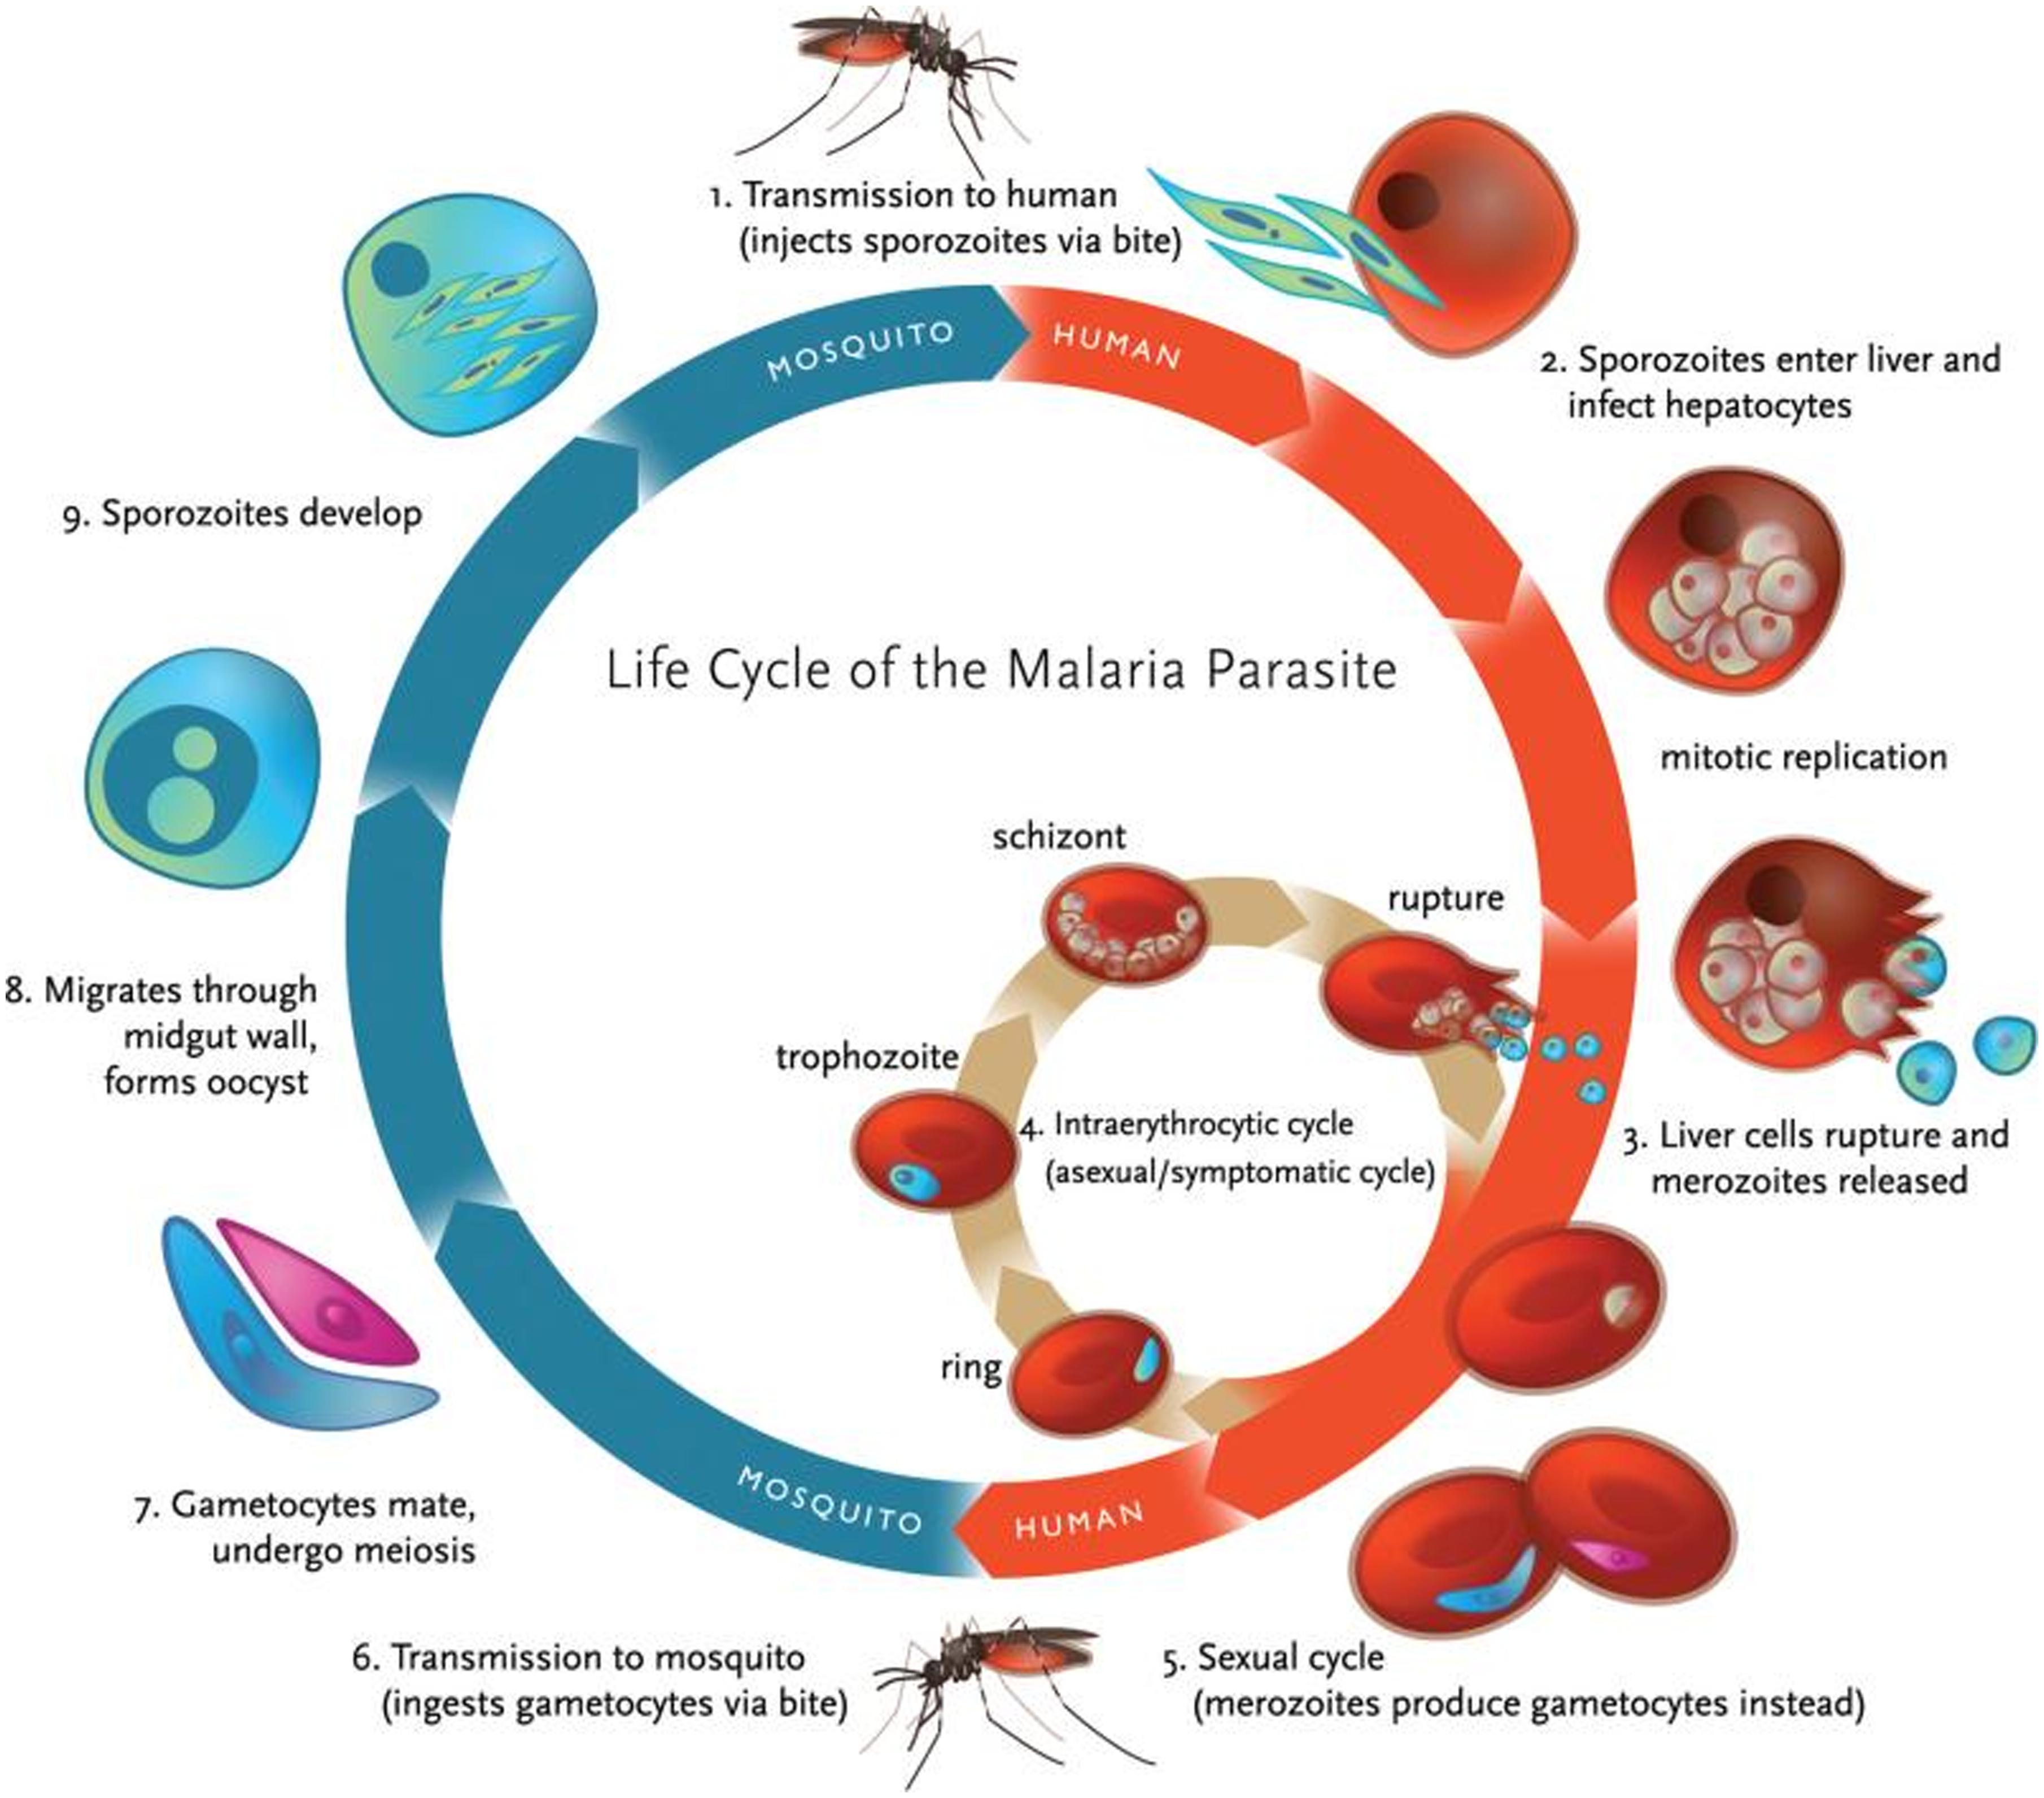
\includegraphics[width=0.75\linewidth]{figures/plasmodium_lifecycle.jpg}
\end{figure}
\end{frame}

% 2. Motivation and experiments
\begin{frame}
\frametitle{How are {\em P. falciparum's} gene expression and 3D structure related?}
{\color{Blue} \textbf{Motivation}}
\begin{itemize}[label={$\bullet$}]

\item One of the main limiting factors for the
development of therapies is the poor understanding of complex gene regulation
of the parasite.
\item The 3D architecture is thought to play an important role in gene
regulation.
\end{itemize}

\vspace{1em}
{\color{Blue} \textbf{Question}} How is the 3D structure of the genome related
to gene expression and regulation?

\vspace{1em}
{\color{Blue} \textbf{Experiment}} We performed Hi-C experiments at five time
points in the lifecycle of the parasite 

\end{frame}

\begin{frame}
\frametitle{3D modeling recapitulates known organizational principles of {\em Plasmodium} genome}
  
\begin{center}
  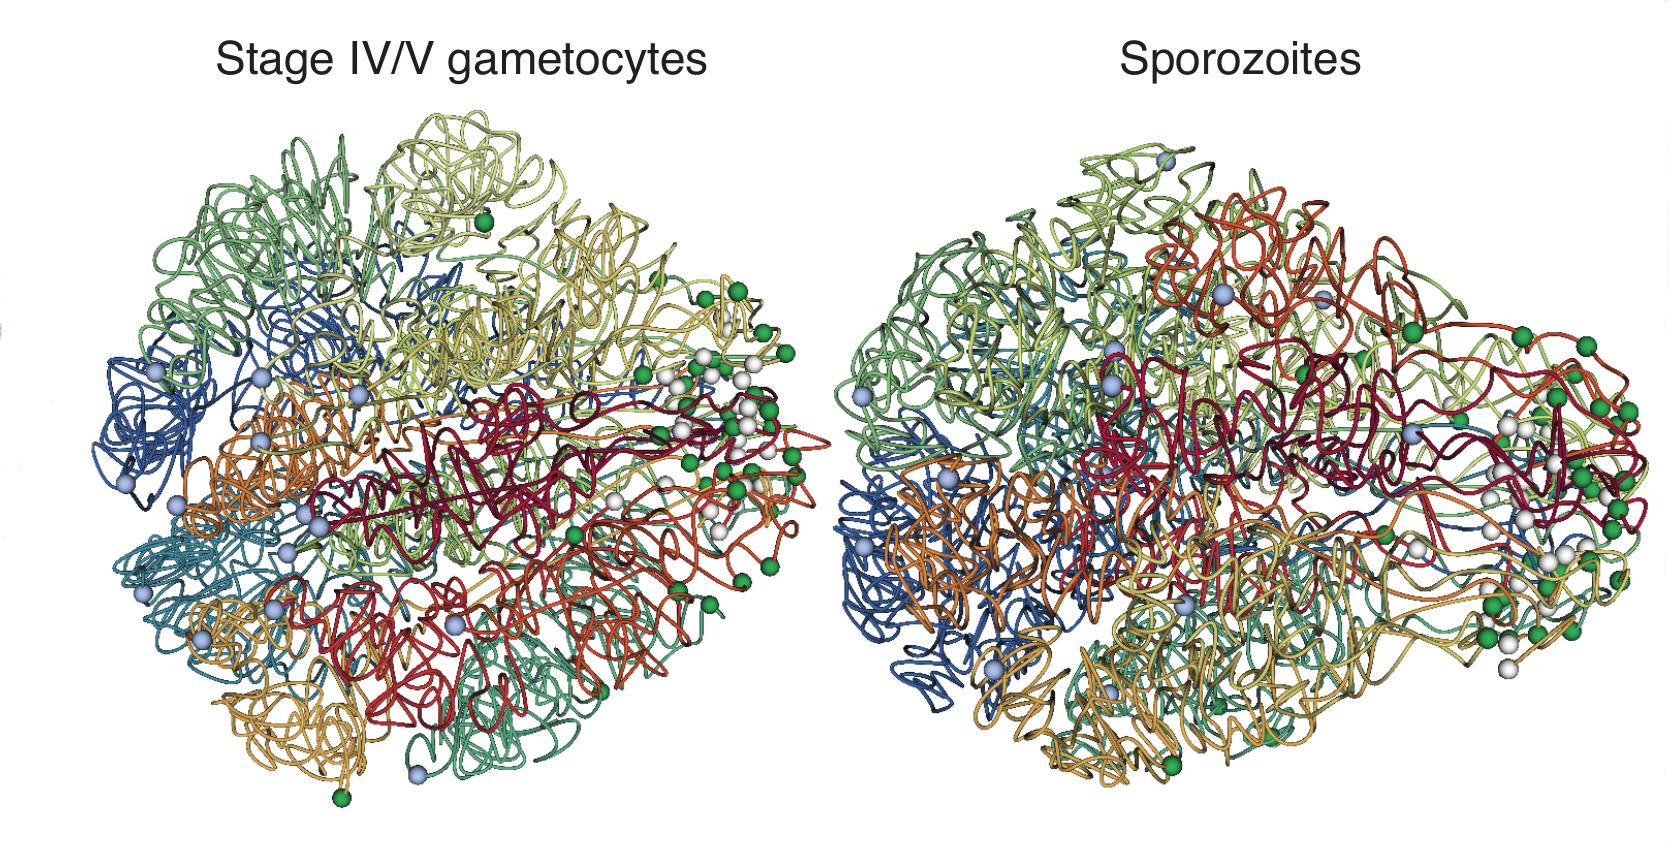
\includegraphics[width=0.95\linewidth]{images/3D_structures_gam_spo.png}
\end{center}
  
\end{frame}
  
  % 4. Validation
  \begin{frame}
  \frametitle{Colocalization of loci is validated with FISH}
  \begin{figure}
  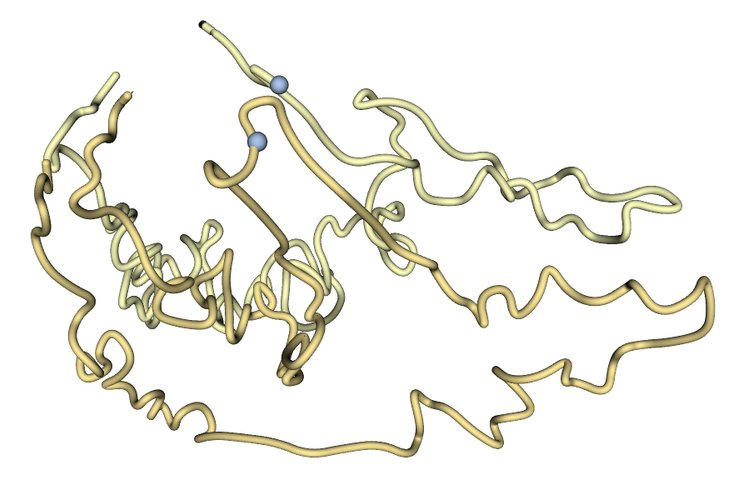
\includegraphics[scale=0.2]{figures/3D_FISH_1.jpg}
  \end{figure}
  \begin{figure}
  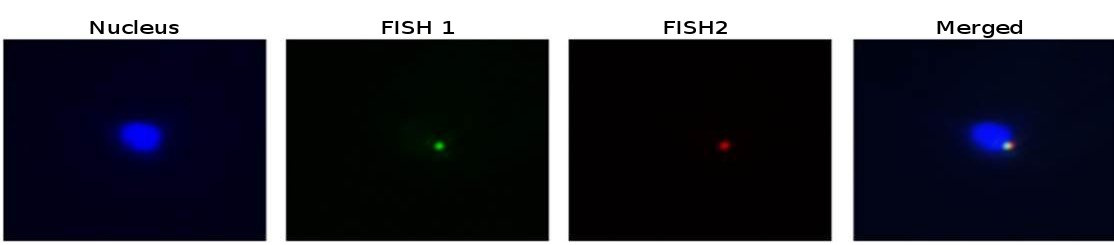
\includegraphics[scale=0.45]{figures/FISH_1.jpg}
  \caption{\textbf{Var genes on chromosomes VII and VIII colocolize}
  }
  \end{figure}
  \end{frame}
  
\begin{frame}
  \frametitle{Identifying links between gene expression profiles and 3D structure}
  {\color{Blue} \textbf{Motivation:}} Extract a gene expression profile
  $v \in \mathbb{R}^p$ that is:
  \begin{itemize}[label={$\bullet$}]

  \item representative of the gene expression profiles ;
  \item correlated with the 3D structure;
  \end{itemize}
  \vspace{1em}
  {\color{Blue} \textbf{Data:}}
  For each gene $g \in \mathcal{G}$
  \begin{itemize}[label={$\bullet$}]
\item Log expression profiles at 27 datapoints: $e(g) = \left( e_1(g), \ldots, e_p(g)\right) \in \mathbb{R}^p$ .
  \item Gene's 3D coordinates, extracted from the inferred 3D structure: $x(g)$.
  \end{itemize}
  \vspace{1em}
  {\color{Blue} \textbf{Method}:}
   KernelCCA \citep{vert:graph, bach:kernel}

  \end{frame}


  \begin{frame}
  \frametitle{Extracting a vector $v$ representative of the gene expression
  profiles}
  Find $v \in \mathbb{R}^p$ to maximize:
  \begin{equation*}\label{eq:variance}
  V(v) = \frac{\sum_{g \in \mathcal{G}} \left(v^T e(g)\right)^2}{\|v\|^2}\,
  \end{equation*}

  \begin{figure}
  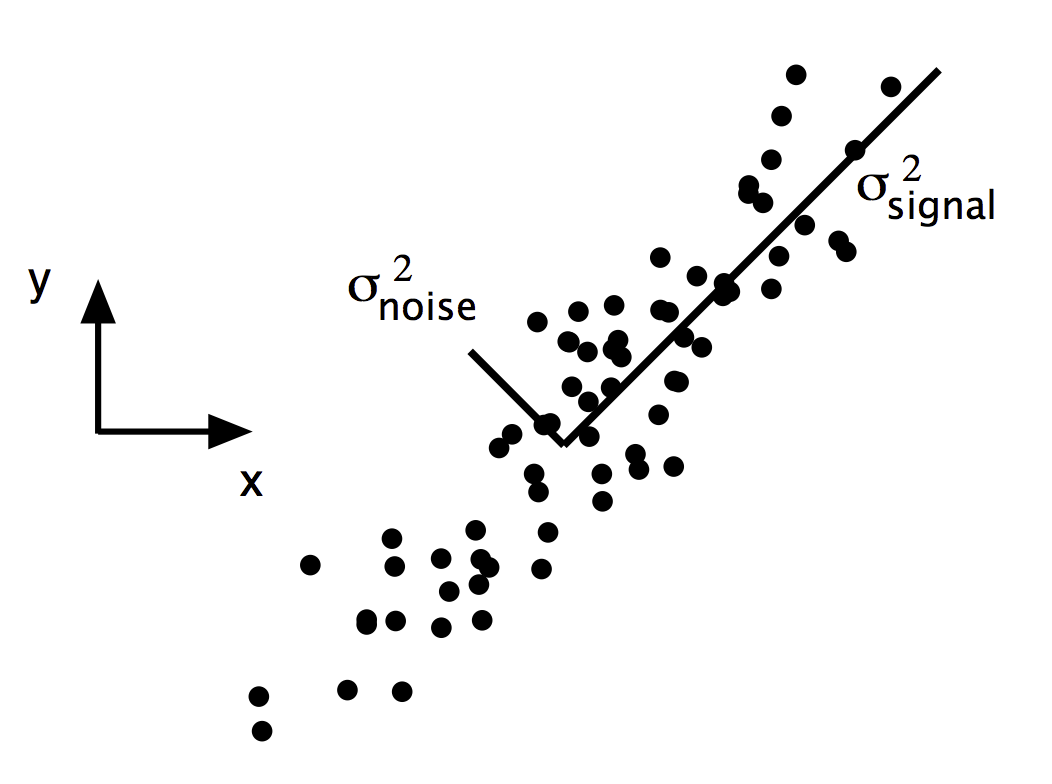
\includegraphics[width=0.5\linewidth]{figures/pca.png}
  \end{figure}
  \end{frame}

\begin{frame}
\frametitle{Find $f$ such that $f$ is smooth with respect to the 3D structure}
  Let $f$ be a vector of scores assigned to each genes. \\

\begin{equation*}\label{eq:smoothness}
  S(f) = \frac{f^\top K^{-1}_{3D} f}{||f||^2}\,
  \end{equation*}

  \vspace{1em}
  We want:
  \begin{itemize}[label={$\bullet$}]
  \item $V(v)$ be large,
  \item $S(f)$ be small,
  \item $\left(v^\top e(g)\right)_{g\in\mathcal{G}}$ and $f$ be as correlated as possible
  \end{itemize}

  \vspace{1em}
  \begin{center}
  {\color{Blue} \bf This can be cast as a generalized eigenvalue problem}
  \end{center}

  \end{frame}


  \begin{frame}
  \frametitle{KernelCCA reveals a strong correlation between gene expression
  profiles and 3D structure}
  \begin{figure}
  \begin{center}
  \includegraphics[width=0.6\linewidth]{images/corr_struture_gene_expression.pdf}
  \end{center}
  \end{figure}
  \end{frame}



\begin{frame}
\Large{ \bf
Functional data analysis for time-course transcriptomic data.}

\begin{flushright}
\vspace{1em}
\small
\textit{joint work with Stephanie Degraaf, the EPICON consortium, and \\
Elizabeth Purdom.}
\end{flushright}
\end{frame}

\begin{frame}
\frametitle{Analysing time-course transcriptomic data}
\footnotesize
\begin{overlayarea}{12cm}{5cm}
\vspace{1em}

{\bf Data:} Timecourse RNAseq data of $\sim$ 400 leaf and root samples of
sorgho under drought stress.

\vspace{1em}
\only<2->{{\bf Problem~:} Biological interpretation is impaired by the shear
amount of genes differentially expressed (95\% of the genes).}

\vspace{1em}
\only<3->{{\bf Goal~:}\quad Develop a clustering method taking in account the
time-course aspect of the data in order to group co-regulated genes.}
\end{overlayarea}

\begin{flushright}
{\tiny {\color{red} Varoquaux$^*$} et al, accepted}
\end{flushright}
\begin{overlayarea}{12cm}{3cm}
{\centering
\begin{center}
\only<1->{
\includegraphics[width=\linewidth]{schemas/epicon_sampling.pdf}}
\end{center}}
\end{overlayarea}
\end{frame}



\begin{frame}
\frametitle{Clustering of time-course gene expression data}

\vspace{-2em}
\only<1>{%
\begin{figure}
\includegraphics[width=0.65\linewidth]{codes/images/splines_data.pdf}
\end{figure}}
\only<2>{%
\begin{figure}
\includegraphics[width=0.65\linewidth]{codes/images/splines_modeling.pdf}
\end{figure}}
\only<3>{%
\begin{figure}
\includegraphics[width=0.65\linewidth]{codes/images/gene_data.pdf}
\end{figure}}
\only<4->{%
\begin{figure}
\includegraphics[width=0.65\linewidth]{codes/images/scaled_centroids.pdf}
\end{figure}
}
\vspace{-1em}
\begin{overlayarea}{12cm}{5cm}
\only<1-4>{%
\vspace{1em}
{\tiny {\color{red} Varoquaux$^*$} et al, accepted}
{\centering
\vspace{2em}

\includegraphics[width=\linewidth]{schemas/epicon_sampling.pdf}}
}
\only<5->{%
{\bf \small Clustering via a constrained mixture model}
\vskip-1.3ex
\rule{\dimexpr\paperwidth-1.5cm\relax}{0.4pt}
}
\only<5>{%
\begin{equation*}
\underbrace{y_{ij}}_{\text{\tiny data}} \quad \sim \quad \sum_k \quad
\underbrace{\pi_k}_{\text{\tiny mixture coefficient}}
\quad \mathcal{N}\large(a_{ik}\underbrace{\mu_k(t_j)}_{\text{\tiny
centroid, $\text{min}\mu(t_j) = 0$, $\text{max}\mu(t_j) = 1$}} +
b_{ik}, \sigma^2_{ikt}\large)
\end{equation*}
}
\only<6->{%
\begin{equation*}
\underbrace{y_{ij}}_{\text{\tiny data}} \quad \sim \quad \sum_k \quad
\underbrace{\pi_k}_{\text{\tiny mixture coefficient}}
\quad \text{ZINB}\large(a_{ik}\underbrace{\mu_k(t_j)}_{\text{\tiny
centroid, $\text{min}\mu(t_j) = 0$, $\text{max}\mu(t_j) = 1$}} +
b_{ik} \large)
\end{equation*}
}
\vspace{-1.5em}
\only<5->{%
\begin{flushright}
\tiny {\color{red} Varoquaux$^*$}, DeGraaf$^*$, Purdom, in prep.
\end{flushright}
}
\end{overlayarea}
\end{frame}

\begin{frame}
\frametitle{Dynamics of gene expression in droughted sorghum plants}
\begin{figure}
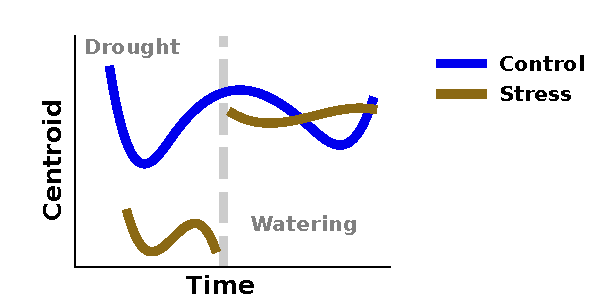
\includegraphics[width=0.6\linewidth]{figures/amf_centroids.pdf}
\end{figure}

\vspace{1.5em}
\begin{overlayarea}{12cm}{5cm}
\only<2->{%
{\bf \small Genes involved in arbuscular mycorrhiza fungi symbiosis}
\vskip-1.3ex
\rule{\dimexpr\paperwidth-1.5cm\relax}{0.4pt}
\begin{figure}
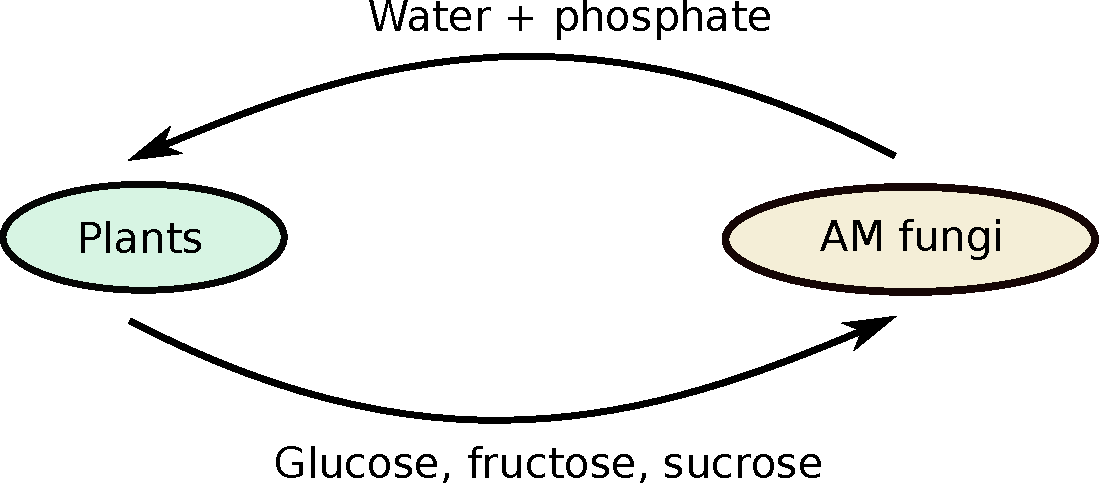
\includegraphics[width=0.5\linewidth]{schemas/symbiose_amf.pdf}
\end{figure}}
\end{overlayarea}
\end{frame}





\begin{frame}
\Large{ \bf
The future…}

\begin{flushright}
\vspace{1em}
\small
Machine learning in high dimension: structures, functions, and regulations of
genomes.

\end{flushright}

\end{frame}


\begin{frame}
\frametitle{Research project}
\vspace{-2em}
\begin{center}
\em
\color{red}
Machine learning in high dimension: structures, functions, and regulations of
genomes.
\end{center}

\begin{overlayarea}{12cm}{5cm}
\small
\only<2->{\textbf{Biological questions}: better understand the regulatory
mecanisms of gene expression}

\only<3->{%
\vspace{1em}
\textbf{Develop high dimensional machine learning tools} for epigenetic data:}

\begin{columns}
\begin{column}{0.7\linewidth}
\begin{itemize}[leftmargin=*]
\footnotesize
\item<4-> {\bf Axis I} \quad Analyse the three-dimensional structure of the
genome.
\item<4->
\item<4->
\item<5-> {\bf Axis II} \quad Mediation analysis in high dimension for
epigenetic data integration and GRN inference.
\end{itemize}
\end{column}
\begin{column}{0.3\linewidth}
\only<4->{%
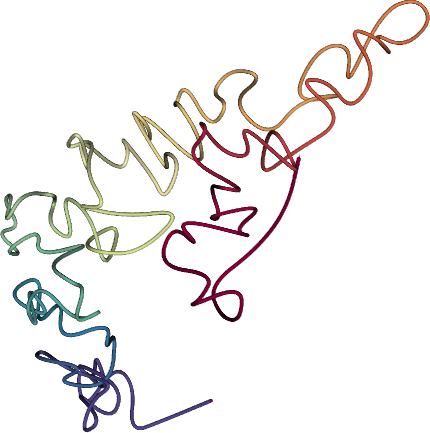
\includegraphics[width=0.5\linewidth]{images/yeast_chr2.png}
}
\begin{overlayarea}{0.9\linewidth}{2cm}
\only<5->{%
\vspace{1em}
\begin{flushright}
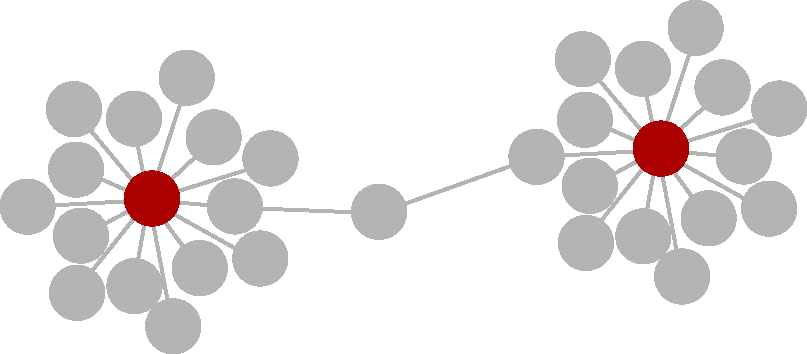
\includegraphics[width=0.8\linewidth]{figures/grn.pdf}
\end{flushright}
}
\end{overlayarea}
\end{column}
\end{columns}
\end{overlayarea}
\end{frame}

\begin{frame}[allowframebreaks,noframenumbering]
  \frametitle{References}
  \bibliographystyle{plainnat}
  \bibliography{biblio}
\end{frame}


\begin{frame}[t, noframenumbering]
\frametitle{Publications}

{\bf \small Publication de rang A, premier auteur}
\vskip-1.3ex
\rule{\dimexpr\paperwidth-1.5cm\relax}{0.4pt}
\begin{itemize}
\small
\item[-] Unfolding the Genome: The Case Study of {\em P. falciparum}. {\color{red}
Varoquaux} (2018)
\item[-] Effective normalization for copy number variation in Hi-C data.
Servant$^*$, {\color{red} Varoquaux$^*$} et al. (2018)
\item[-] Accurate identification of centromere locations in yeast genomes
using Hi-C. {\color{red} Varoquaux} et al. (2015)
\item[-] A statistical approach for inferring the 3D structure of the genome.
{\color{red} Varoquaux} (2014)
\item[-] Three-dimensional modeling of the P. falciparum genome during the
erythrocytic cycle reveals a strong connection between genome architecture and
gene expression. Ay, Bunnik, {\color{red} Varoquaux$^*$} et al. (2014)
\end{itemize}
\end{frame}

\begin{frame}[t, noframenumbering]
\frametitle{Publications}

{\bf \small Publication de rang A, deuxième auteur}
\vskip-1.3ex
\rule{\dimexpr\paperwidth-1.5cm\relax}{0.4pt}
\begin{itemize}
\small
\item[-] The Types, Roles, and Practices of Documentation in Data Analytics
Open Source Software Libraries. Geiger, {\color{red} Varoquaux} et al. (2018)
\item[-] HiC-Pro: an optimized and flexible pipeline for Hi-C data processing.
\quad Servant, {\color{red} Varoquaux} et al. (2015)
\end{itemize}

{\bf \small Autres publications de rang A}
\vskip-1.3ex
\rule{\dimexpr\paperwidth-1.5cm\relax}{0.4pt}
\begin{itemize}
\small
\item[-] Changes in genome organization of parasite-specific gene families
during the Plasmodium transmission stages. \quad Bunnik$^*$, Cook$^*$,
{\color{red} Varoquaux} et al. (2018)
\item[-] Identifying multi-locus chromatin contacts in human cells using
tethered multiple 3C. Ay, Vu, Zeitz, {\color{red} Varoquaux} (2015)
\item[-] A community effort to assess and improve drug sensitivity prediction
algorithms. Costello et al. (2014)
\end{itemize}
\end{frame}

\begin{frame}[t, noframenumbering]
\frametitle{Publications}
{\bf \small Autres publications}
\vskip-1.3ex
\rule{\dimexpr\paperwidth-1.5cm\relax}{0.4pt}
\begin{itemize}
\small
\item[-] Measuring cluster stability for bayesian non-parametrics using the
linear bootstrap
\item[-]
\end{itemize}

{\bf \small Publications soumises}
\vskip-1.3ex
\rule{\dimexpr\paperwidth-1.5cm\relax}{0.4pt}
\begin{itemize}
\item[-] Lifecycle transcriptomics of field-droughted sorghum reveals rapid
biotic and metabolic responses. \quad {\color{red} Varoquaux$^*$}, Cole$^*$,
Gao$^*$ et al. 
\item[-] FIXME pipeline paper
\item[-] JOSS
\end{itemize}

{\bf \small Publications en cours de rédaction}
\vskip-1.3ex
\rule{\dimexpr\paperwidth-1.5cm\relax}{0.4pt}
\begin{itemize}
\item[-] jupyter
\item[-] documentation
\item[-] FOSS with Alex
\item[-] Clustering
\item[-] NB structure
\item[-] Diploid
\end{itemize}
\end{frame}

\begin{frame}[t, noframenumbering]
\frametitle{}
\end{frame}

\end{document}

